\chapter[Estágio]{Estágio}

\section{Descrição da Empresa}

Happe Soluções em Tecnologia, CNPJ 22.063.980/0001-04, situada no Edíficio Ipanema,
SHIS QI 09, Bloco U, Sala 201, Lago Sul, Brasília - DF, CEP 71625-095.

Empresa referência em serviços que englobam desde o desenvolvimento tecnológico
de soluções de novas idéias, serviços de plataformas próprias até a consultorias e integrações
com sistemas já implantados. A empresa foi fundada por dois engenheiros da computação
e já atua de forma consolidada no mercado a mais de 2 anos.

\section{Atividades Desenvolvidas}

As atividades desenvolvidas durante a realização do estágio englobam todo o ciclo
de vida da Engenharia de Software para o desenvolvimento de uma aplicação web.

O escopo da aplicação envolve um portal de gerenciamento de conteúdo a ser utilizado
pela Associação dos Médicos Peritos da Previdência Social (ANMP).

A aplicação envolve algumas features principais, a seguir as features são detalhadas
com imagens do próprio produto desenvolvido.

\textbf{Seção de Sliders}


\includegraphics[keepaspectratio=true,scale=0.3]{figuras/banners.png}

\textbf{Seção de Notícias}

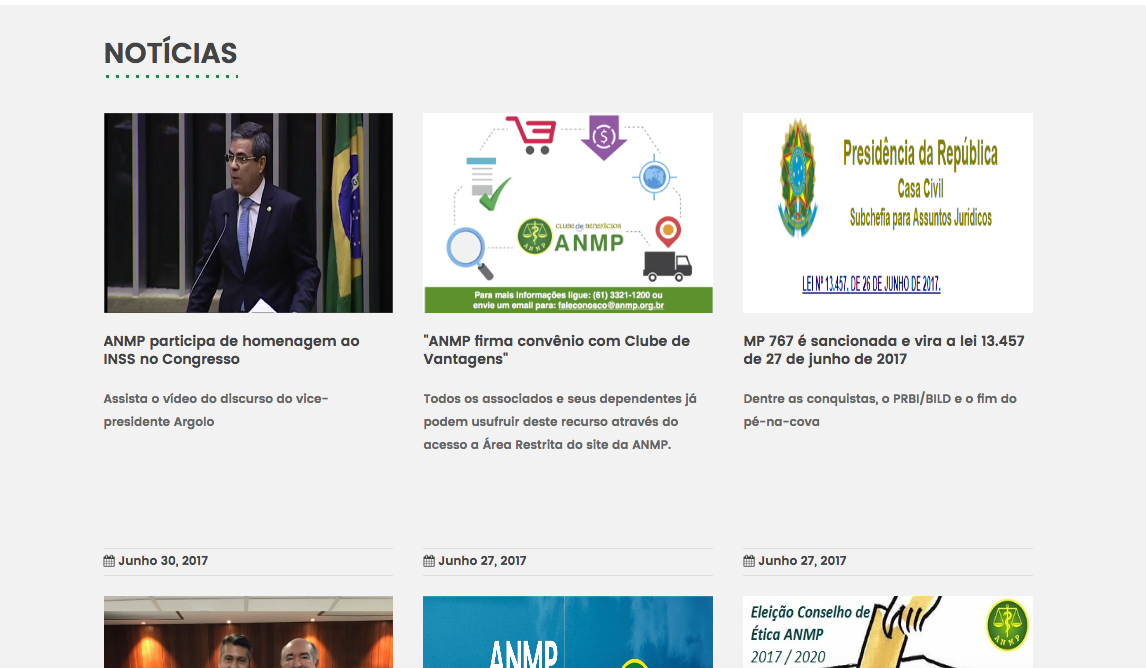
\includegraphics[keepaspectratio=true,scale=0.3]{figuras/noticias.png}

\textbf{Seção de Vídeos}

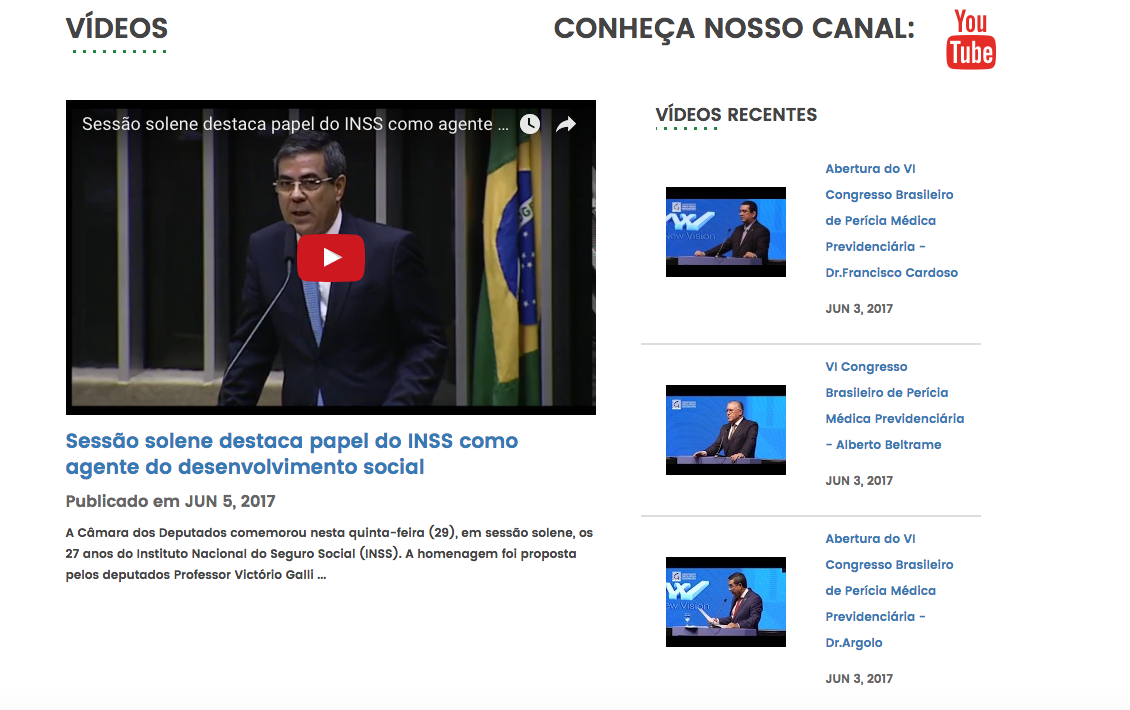
\includegraphics[keepaspectratio=true,scale=0.3]{figuras/videos.png}

\textbf{Login}

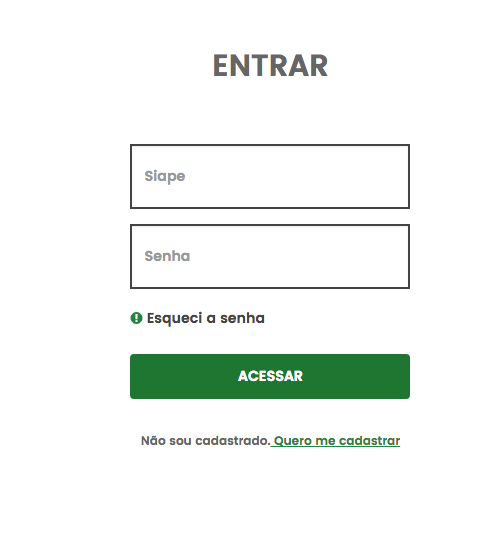
\includegraphics[keepaspectratio=true,scale=0.3]{figuras/login.png}

\textbf{Cadastro}

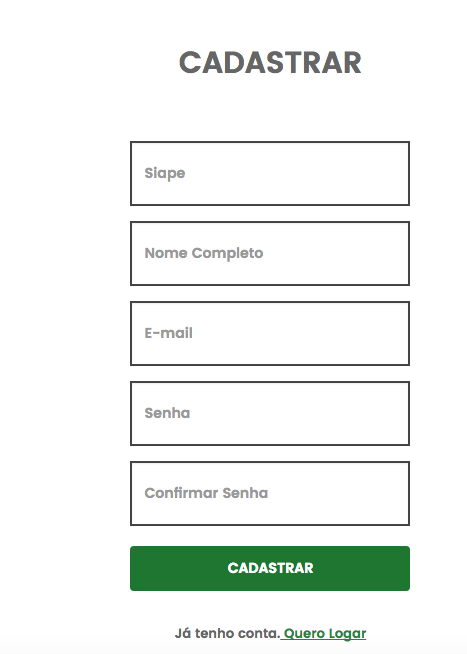
\includegraphics[keepaspectratio=true,scale=0.3]{figuras/cadastro.png}

\textbf{Contato}

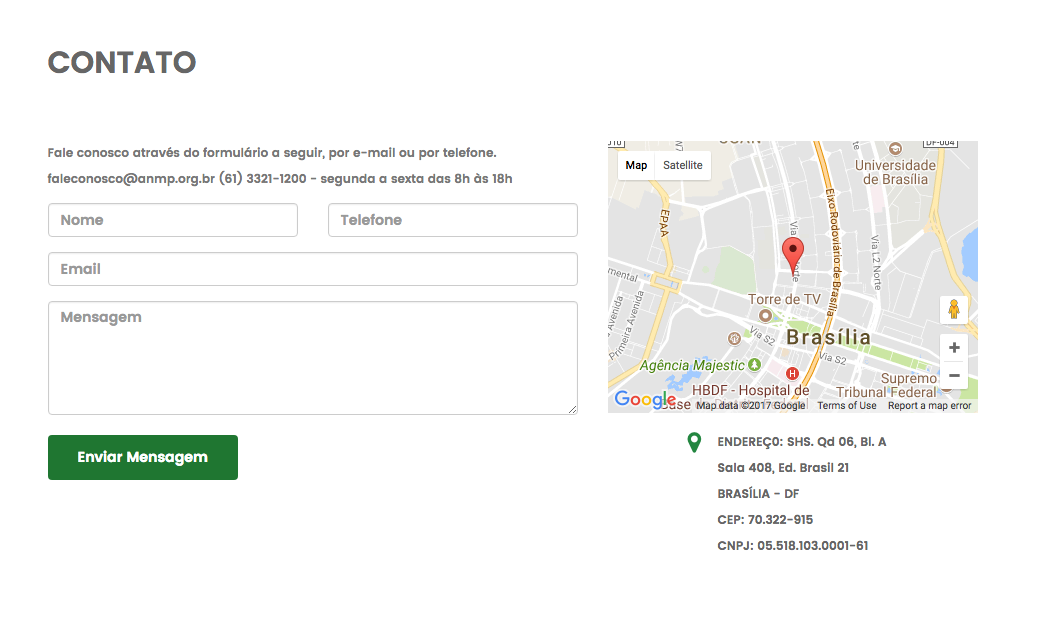
\includegraphics[keepaspectratio=true,scale=0.3]{figuras/contato.png}

\textbf{Quem Somos}

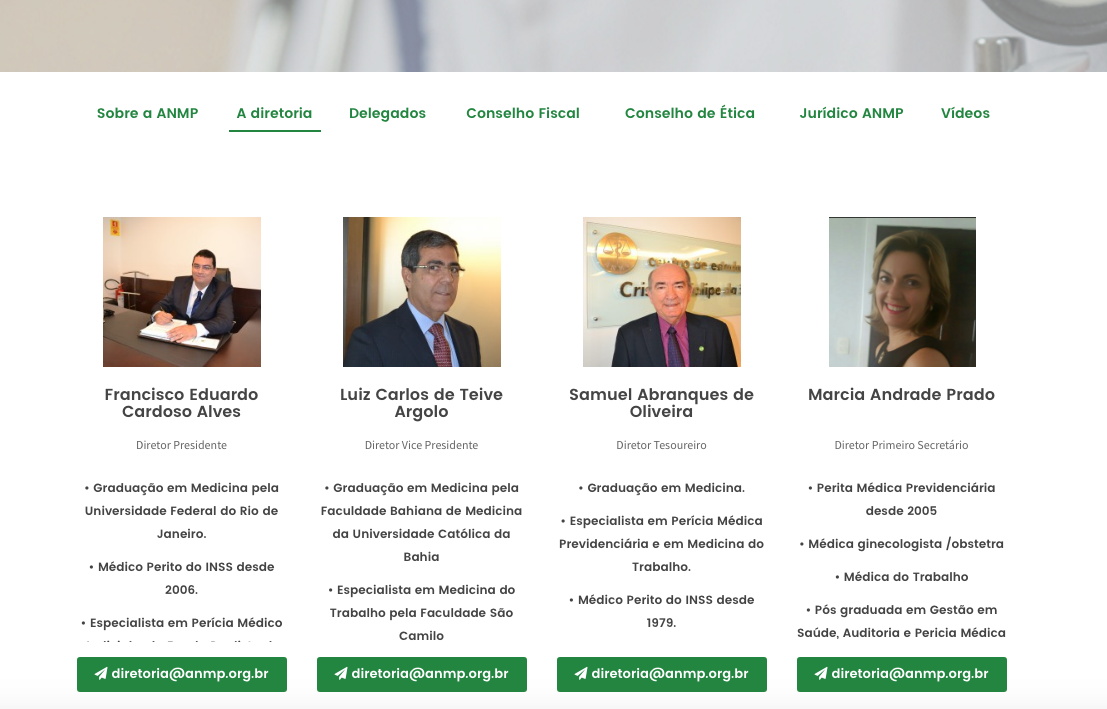
\includegraphics[keepaspectratio=true,scale=0.3]{figuras/quem.png}

\textbf{Sobre}

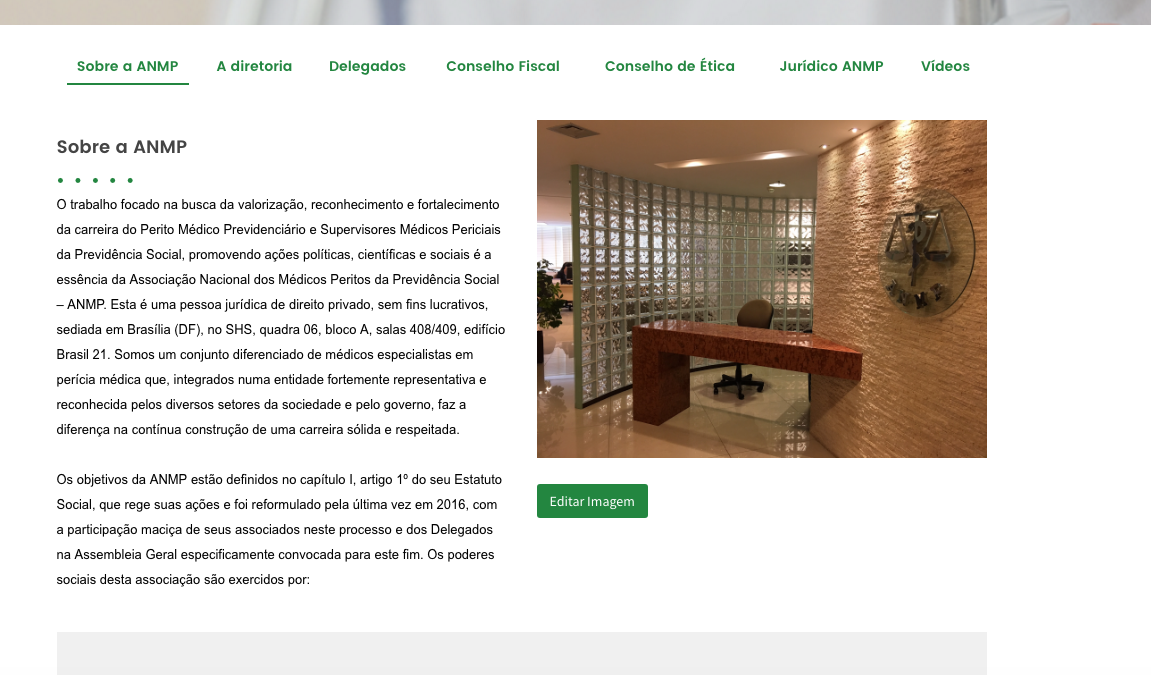
\includegraphics[keepaspectratio=true,scale=0.3]{figuras/sobre.png}

\textbf{Notícias}

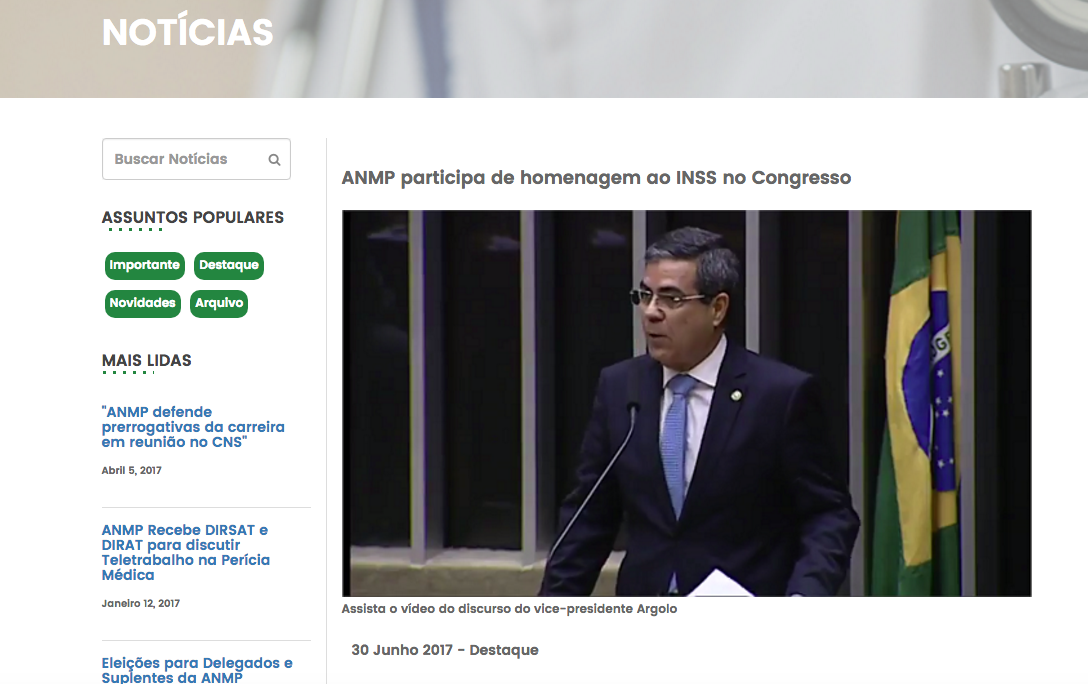
\includegraphics[keepaspectratio=true,scale=0.3]{figuras/nots.png}

\textbf{Interno}

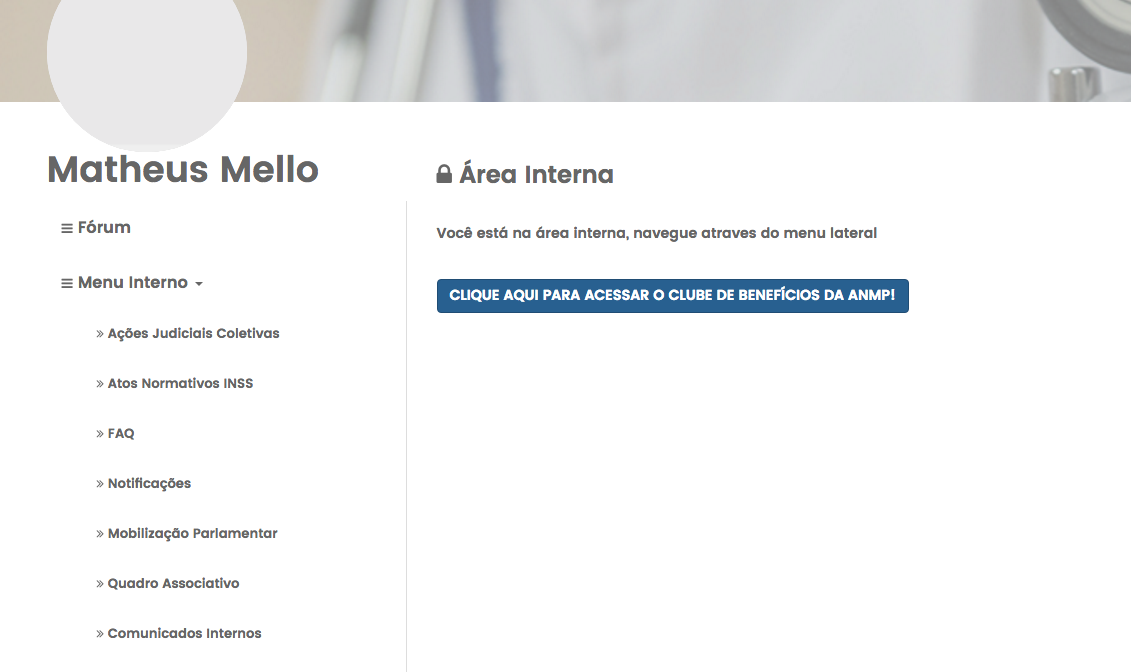
\includegraphics[keepaspectratio=true,scale=0.3]{figuras/interno.png}

\textbf{Fórum}

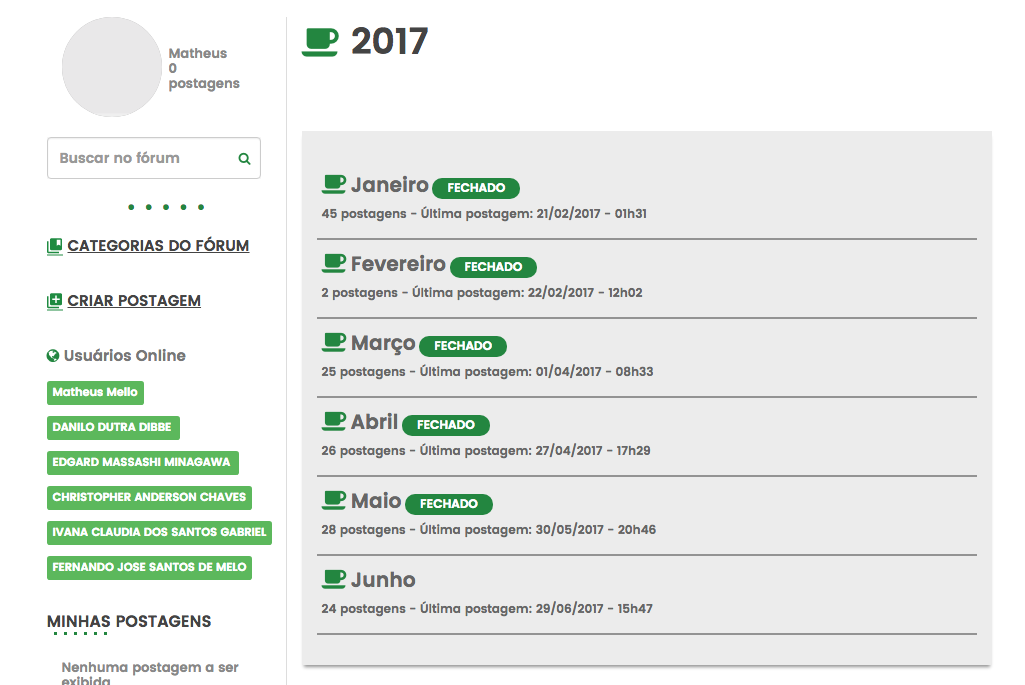
\includegraphics[keepaspectratio=true,scale=0.3]{figuras/forum.png}

\textbf{Dashboard de Administração}

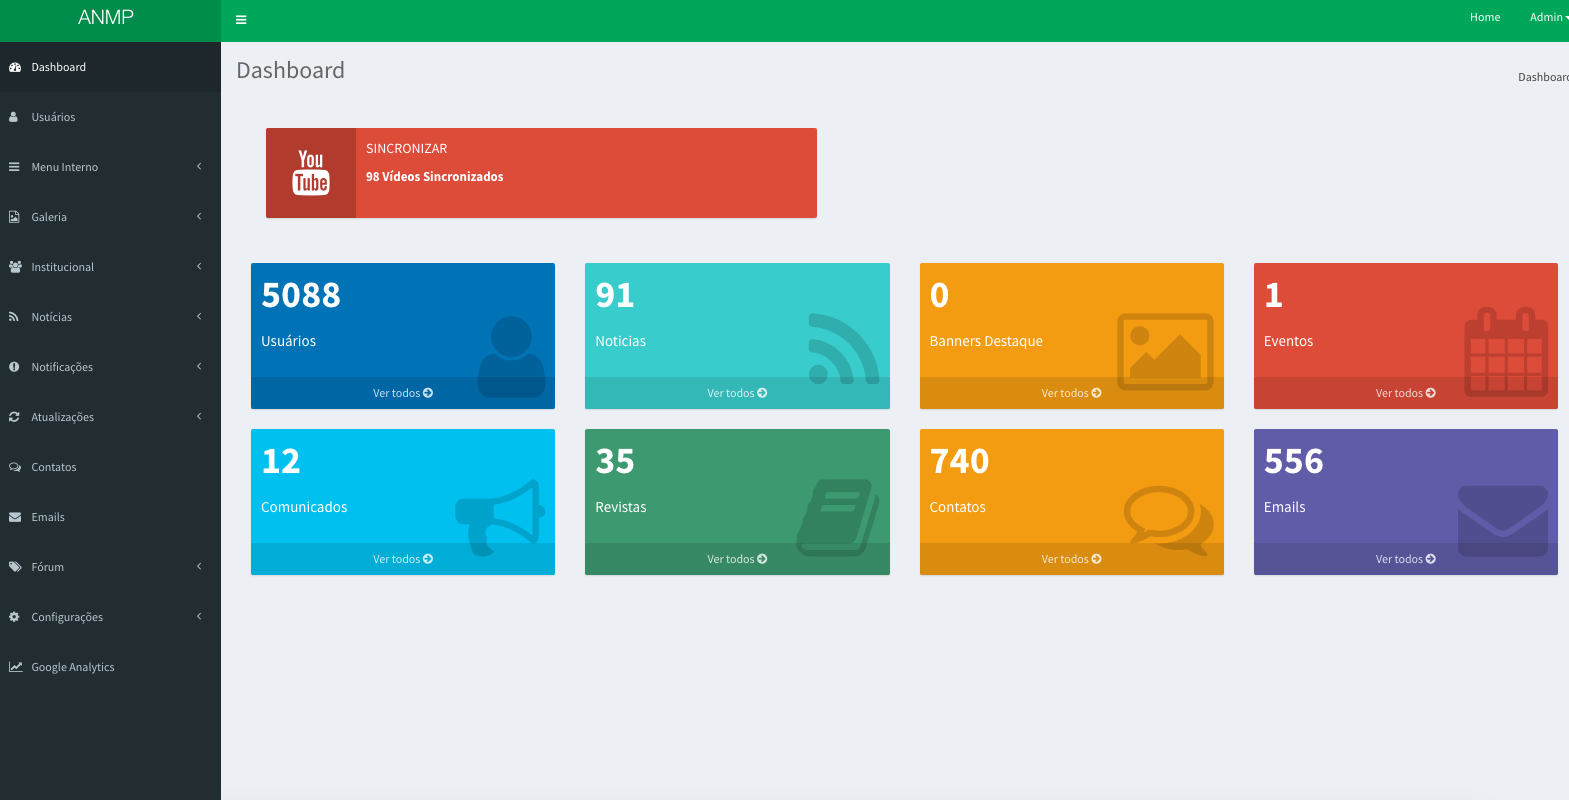
\includegraphics[keepaspectratio=true,scale=0.3]{figuras/admin.png}

Matheus Mello Nascimento atuou como Desenvolvedor Web Full-Stack, utilizando
Node.JS. Matheus teve experiência com todo o fluxo da engenharia de software, utilizando o SCRUM.
Tendo contato direto com os clientes ou donos do projeto. Fazendo parte desde seu planejamento, com a criação
de histórias de usuário e estimativas, até o desenvolvimento e testes do software.

Também foi utilizada a técnica de daily SCRUM, caracterizando-se por reuniões diárias de equipe e semanais ou quinzenais com os stakeholders.



% 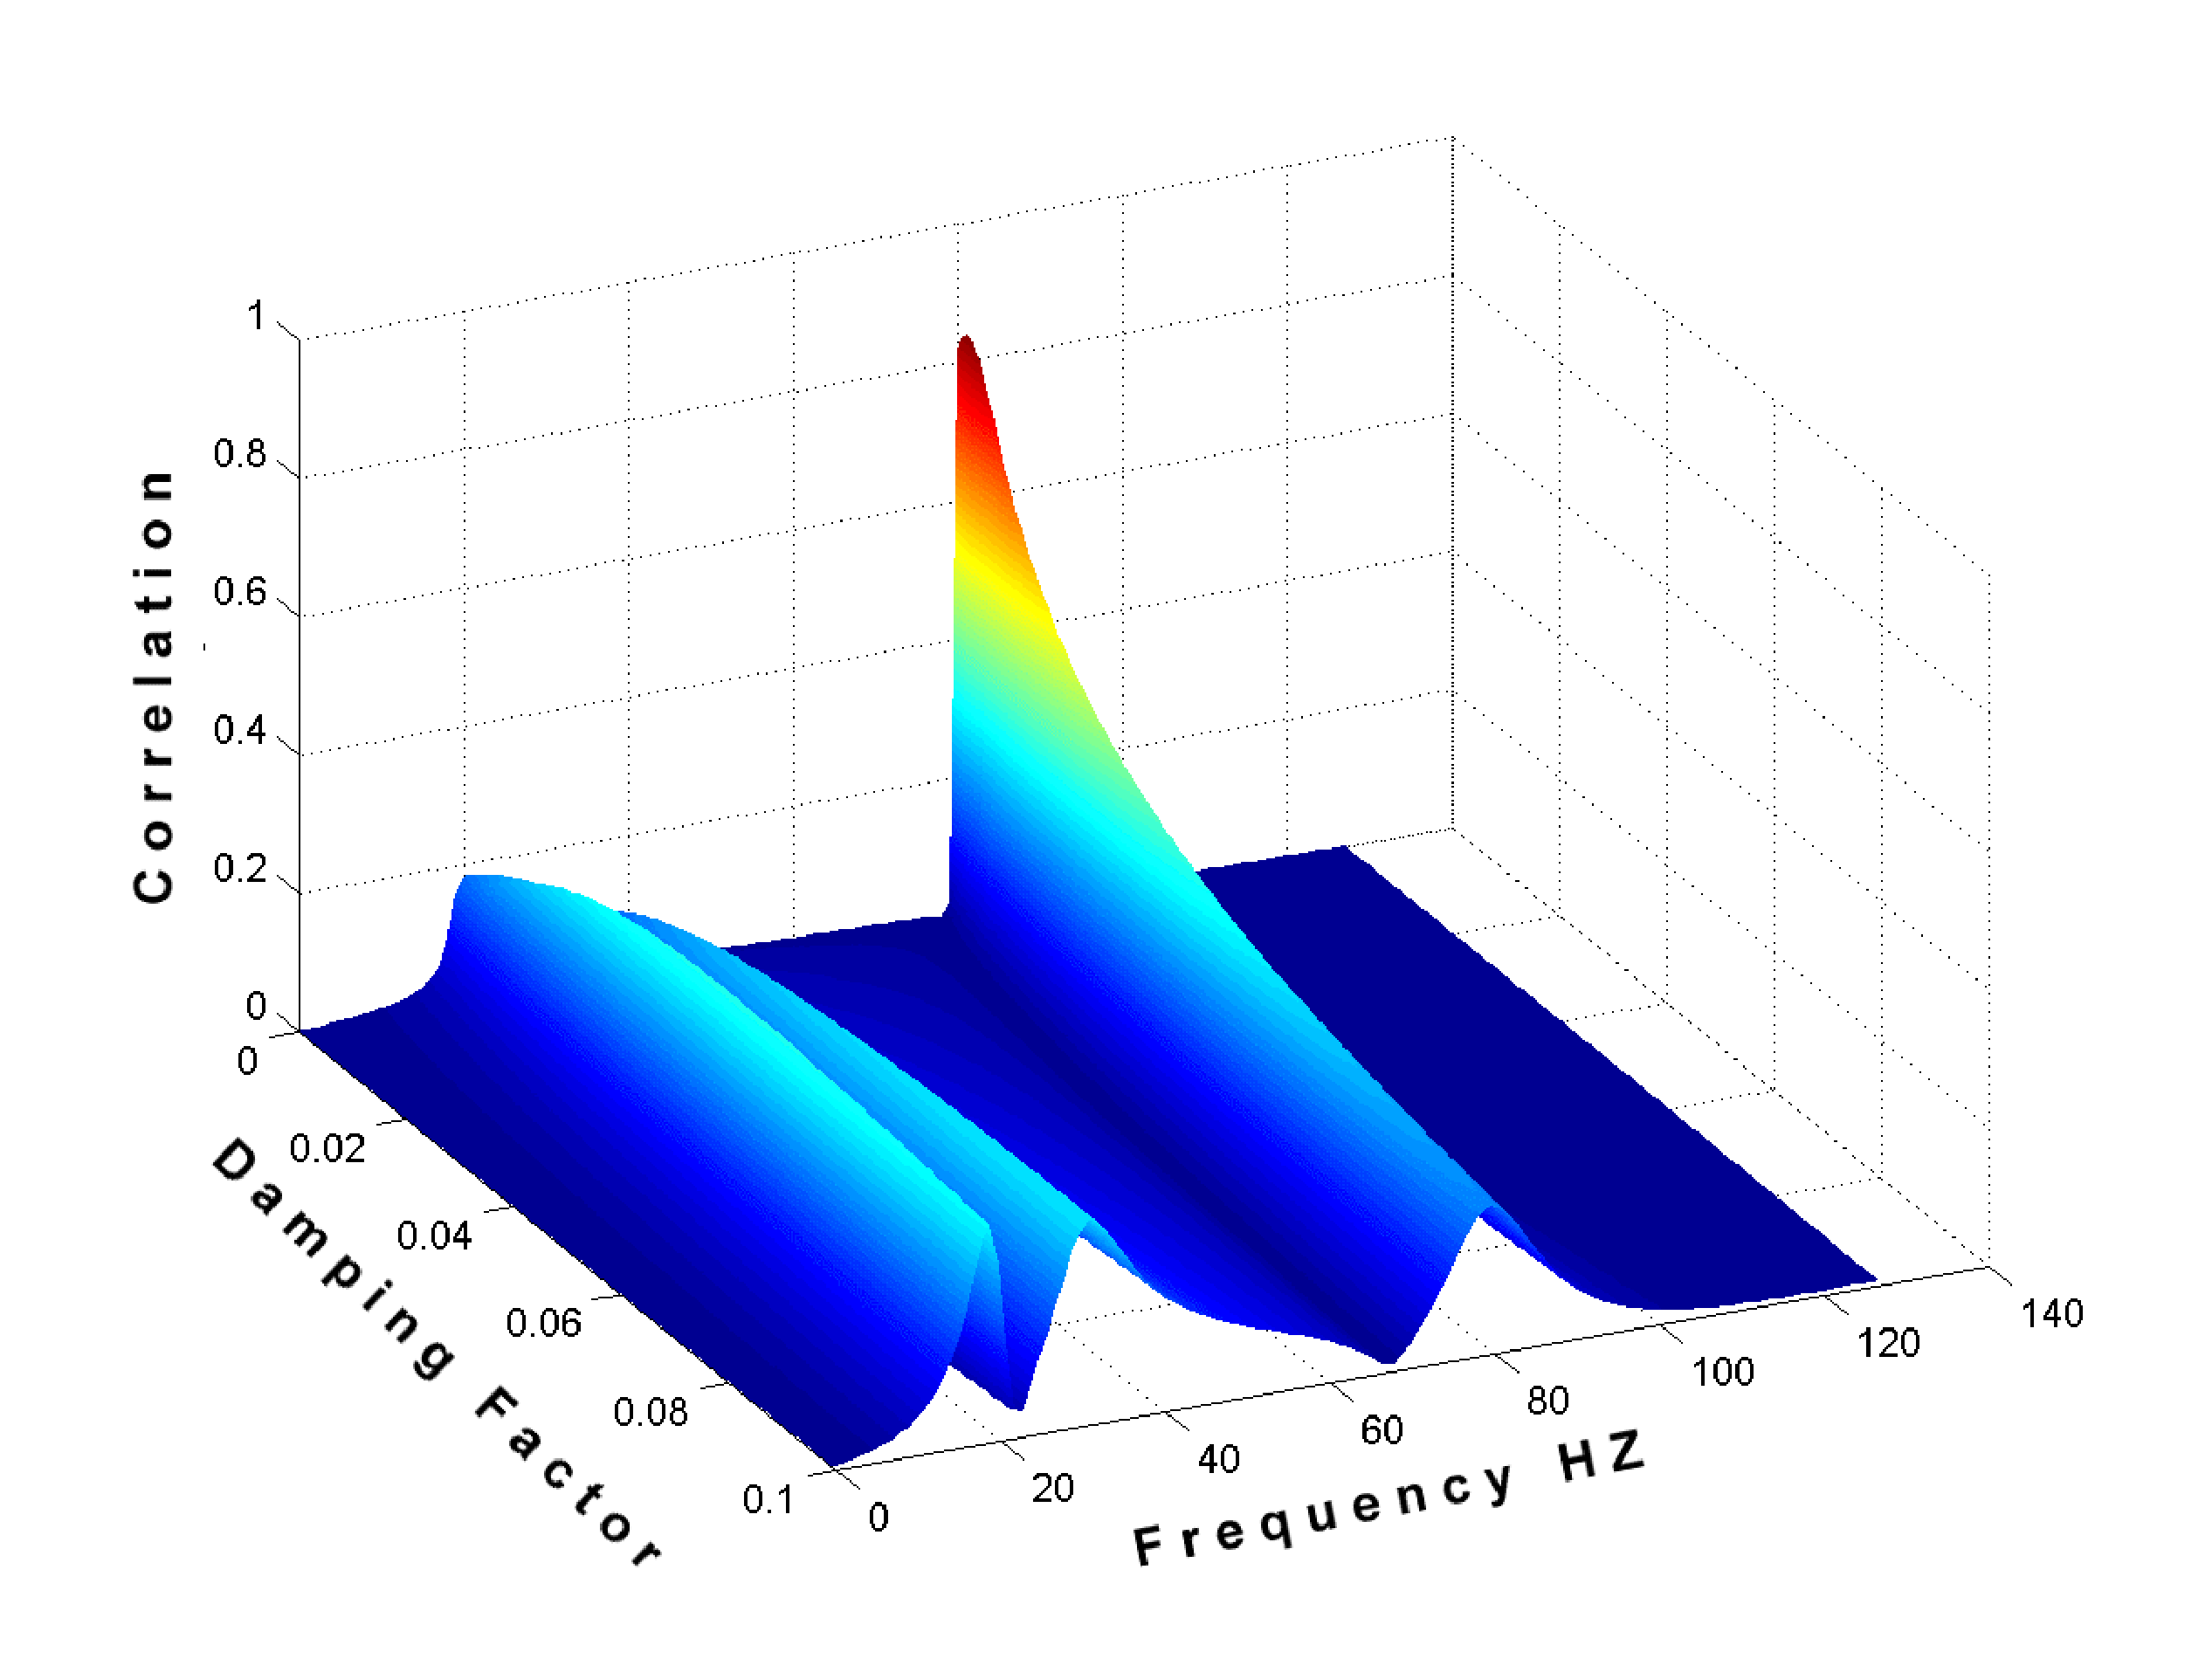
\includegraphics[keepaspectratio=true,scale=0.3]{figuras/fig01.eps}


% \subsection{Objetivos Gerais}
% \subsection{Objetivos Específicos}
% \section{Metodologia}
% \section{Organização}
